\chapter{Dise\~no de la soluci\'on}

% **************************** Define Graphics Path **************************
\ifpdf
    \graphicspath{{Chapter3/Figs/Raster/}{Chapter3/Figs/PDF/}{Chapter3/Figs/}}
\else
    \graphicspath{{Chapter3/Figs/Vector/}{Chapter3/Figs/}}
\fi

En este cap\'itulo se exponen las principales caracter\'isticas relacionadas al dise\~no de la soluci\'on alcanzada. A su vez se exponen, de los problemas y decisiones de dise\~no encontrados aquellos que a nuestro entender resultan m\'as interesantes de mencionar en este cap\'itulo. 
 
\section[Enfoque utilizado]{Enfoque utilizado}

En el cap\'itulo dedicado al estado del arte de las redes definidas por software, se explica en profundidad la arquitectura de SDN, y a partir del mismo queda completamente sanjada la diferencia entre los conceptos de SDN y OpenFlow por ejemplo.\\

Entonces, la primer decisi\'on de dise\~no importante a tener en cuenta es por cual implementaci\'on del enfoque SDN optar, puesto que las alternativas existentes son bien diferentes.\\
 
La respuesta a esta pregunta es sencillamente OpenFlow en su versi\'on 1.3; y el porque lo explicamos a continuaci\'on.

Dentro de las arquitecturas e implementaciones que se ajustan al enfoque propuesto por SDN, como se menciona en el estado del arte existen varias y una de ellas, y quiz\'as la que m\'as ha tracendido es OpenFlow.\\
OpenFlow cuenta con un nivel de desarrollo bastante bueno, siendo la \'ultima versi\'on comercial liberada al momento de culminar este trabajo la versi\'on 1.5.
A su vez, cuenta con un extensa comunidad de usuarios y es utilizado en varias soluciones comerciales y productos de software relacionados entre los cuales podemos destacar Open vSwitch entre otros. Estos han contribuido a generar una gran cantidad de documentaci\'on y material accesible en la web, los cuales entre otras razones posicionan a OpenFlow como una de las mejores alternativas para el dise\~no del protot\'ipo. En particular [nombrar algunas soluciones tecnologicas que usarn OpenFlow].
Finalmente se puede agregar que OpenFlow esta integramente desarrollado bajo la filosof\'ia Open Source.\\

Por otro lado en las sucesivas versiones de OpenFlow, se han incorporado diferentes caracter\'isticas y funcionalidades que hacen en la actualidad a la versi\'on 1.5 de OpenFlow, una alternativa vers\'atil, flexible y completa.\\

Tomada la decisi\'on de utilizar OpenFlow para la implementaci\'on del prototipo, resta decidir en relaci\'on a esto que versi\'on utilizar del mismo.\\
Como mencionamos anteriormente al momento de culminar el desarrollo de este trabajo, la versi\'on m\'as reciente de OpenFlow era la 1.5; mientras que al momento de iniciado el desarrollo de este proyecto la versi\'on m\'as reciente era la 1.4.\\

Por otro lado dentro de las versiones disponibles de OpenFlow, se tiene que optar por aquella que cumpla con ciertas restricciones a las que el diseni\~no del prototipo esta sujeto; las m\'as importantes y que impactan en esta decis\i'on son:
\begin{itemize}
\item Soporte para MPLS, tanto en la capacidad de reconocer los cabezales MPLS como para la manipulaci\'on de los mismos mediante las primitivas POP, PUSH y SWAP
\item Soporte para tags de VLAN (esta ultima no se si ponerla)
\end{itemize}
Sobre la primer restricci\'on, OpenFlow brinda soporte completo para MPLS a partir de la versi\'on 1.3. Por otro lado en relaci\'on a la segunda restricci\'on [COMPLETAR].\\
Por ello, la versi\'on m\'as b\'asica de OpenFlow que da soporte a las restricciones de dise\~no mencionadas es la versi\'on 1.3.\\

M\'as adelante veremos en la siguiente secci\'on, que esta destinada a la programaci\'on de la placa NetFPGA, que es de inter\'es trabajar con la versi\'on de OpenFlow m\'as sencilla y minimalista que soprte todas las funcionalidades y restricciones impuestas sobre el protot\'ipo. Entonces la versi\'on de OpenFlow a utilizar es la 1.3.

\section[Alternativas de dise\~no para el router]{Alternativas de dise\~no para el router}

Como se menciona anteriormente en este informe, una de las premisas para la elaboraci\'on del router open source es la utilizaci\'on del hardware NetFPGA. A su vez, partiendo de este hardware es necesario llegar a un dispositivo o switch compatible con OpenFlow.\\ 

Existen dos estrategias bien definidas para la construcci\'on un switch OpenFlow, partiendo del hardware mencionado, y utilizando los diferentes proyectos disponibles para la programaci\'on del mismo. Una de ellas es programar el hardware para que se comporte como un switch compatible con el protocolo OpenFlow. La otra alternativa es programar el hardware para que se comporte como una tarjeta de red estandar, e implementar todo el comportamiento de un switch OpenFlow en software.\\

Para la primer estrat\'egia se cuenta con un proyecto desarrollado previamente para la plataforma NetFPGA, y disponible libremente en el repositorio de software de dicho producto. No obstante este proyecto presenta una dificultad y es que a pesar de haber sido dise\~ado para soportar en un futuro cualquier versi\'on disponible del protocolo OpenFlow, en su veri\'on actual solamente soporta un conjunto reducido de funcionalidades de la versi\'on 1.0 de este protocolo. \\
Como se mencion\'o anteriormente la versi\'on m\'as b\'asica de este protocolo que permite soportar el conjunto de funcionalidades relevadas como requerimientos para este proyecto es la versi\'on 1.3. Esto conlleva a la ncesidad de extender el proyecto existente, para soprtar las nuevas caracter\'isticas incorporadas en las sucesivas versiones posteriores a la 1.0; o al menos aquellas que son escenciales para soportar las caracter\'isticas pretendidas sobre el prototipo.\\

Para la segunda estrat\'egia se cuenta con un proyecto tambi\'en desarrollado previamente para la plataforma NetFPGA, llamado ReferenceNIC. Este proyecto habilita a programar el hardware para que se comporte como una placa de red estandar. Adicionalmente se debe incluir o desarrollar herramientas que permitan implementar por software el comportamiento de un switch OpenFlow. En particular sobre este \'ultimo punto vale la pena destacar la existencia de Open vSwitch, herramienta que entre otras caracter\'isticas realiza esto mismo, utilizando hardware tradicional como una placa de red estandar.

Contextualizando ambas alternativas en el marco de la realizaci\'on de este proyecto de fin de carrera, ambas alternativas presentan sus ventajas y desventajas; no siendo ninguna de ellas a priori mejor que la otra. Por ello a continuaci\'on se exponen comparativamente las principales ventajas y desventajas de cada alternativa, a modo de sustentar la elecci\'on de una ellas. 

\newpage
%%% Tabla Ventajas y Desventajas de ambas alternativas
\begin{table}[!Ht]\centering\small
\begin{tabularx}{\textwidth}{|>{\setlength\hsize{1.0\hsize}\setlength\linewidth{\hsize}}X|>{\setlength\hsize{1.0\hsize}\setlength\linewidth{\hsize}}X|}
\hline
\multicolumn{2}{|c|}{Ventajas}\\ \hline 
\hline
Extender proyecto OpenFlow NetFPGA & ReferenceNIC + Open vSwitch\\
\hline
\begin{itemize}
\item \'Optimo aprovechamiento de la capacidad de c\'omputo y procesamiento del hardware disponible.
\item Mayor posibilidad de lograr velocidades de procesamiento competitivas con productos comerciales similares.
\item Mayor posibilidad de obtener resultados aceptables, en performance y rendimiento para puesta en producción.

\end{itemize}
&
\begin{itemize}
\item No se tiene la necesidad de modificar o desarrollar software en el lenguaje y en el entorno de programaci\'on de la tarjeta NetFPGA.

\item Evitar desarrollar software para la NetFPGA ahorra tiempo de proyecto que se puede invertir en otras l\'ineas de trabajo, igualmente importantes. 

\item Programar el harware NetFPGA con proyectos precompilados como el ReferenceNIC requiere \'unicamente de licencias de software que son accesibles sin costo ya sea mediante licencias gratuitas o de prueba.
\end{itemize}
\\
\hline
\end{tabularx}
\end{table}

\begin{table}[!HT]\centering\small
\begin{tabularx}{\textwidth}{|>{\setlength\hsize{1.0\hsize}\setlength\linewidth{\hsize}}X|>{\setlength\hsize{1.0\hsize}\setlength\linewidth{\hsize}}X|}
\hline
\multicolumn{2}{|c|}{Desventajas}\\ \hline
\hline
Extender proyecto OpenFlow NetFPGA & ReferenceNIC + Open vSwitch\\
\hline
\begin{itemize}

\item Extender el proyecto existente, en si mismo constituye un empresa del porte de un proyecto de fin de carrera
\item El conocimiento técnico necesario se perfila m\'as al de un Ingeniero Eléctrico que al de un Ingeniero en Computación, lo cual constituye un riesgo del proyecto.
\item Desarrollar software para el hardware NetFPGA y compilarlo requiere de licencias de software costosas.
\end{itemize}

&

\begin{itemize}
\item No se aprovecha de forma óptima las capacidades de procesamiento del hardware disponible. En otras palabras se tiene hardwre ``caro'' y potente en forma ociosa.
\item Los resultados obtenidos en relaci\'on al rendimiento del prototipo, muy probablemente no sean los esperados para una equipo de producción.
\end{itemize}
\\
\hline
\end{tabularx}
\end{table}

\clearpage
\newpage
Habiendo presentado las principales ventajas y desventajas de cada alternativa, y teniendo presente el alcance y el tiempo disponible para la ejecuci\'on de este proyecto, se opt\'o por la segunda estrat\'egia presentada.\\

Optando por la segunda estrat\'egia presentada se logra obtener de forma temprana un prototipo de switch OpenFlow con el cual trabajar en la programaci\'on del datapath mediante un controlador, desarrollar estrategias para constru\'ir servicios en una red h\'ibrida IP/MPLS, as\'i como dise\~nar pruebas y un testbed acorde para validar tecnol\'ogicamente la soluci\'on propuesta.\\ 


\section[Alternativas de dise\~nio]{Plano de Control centralizado vs distribu\'ido}

\section[Dise\~no general del prototipo]{Dise\~no general del prototipo}

En esta secci\'on se presenta a modo de resumen de las anteriores secciones, la estructura general que adopta la soluci\'on planteada, al asumir todas las decisiones de dise\~no discutidas anteriormente.\\

Comenzando con la estructura del router open source, en ~\ref{fig:OpenSourceRArch} puede apreciarse las principales componentes que lo constituyen; tanto a nivel de hardware como de software.\\
Enfocandos\'e en las componentes del hardware, el router se compone de una PC de escritorio convencional, y una tarjeta NetFPGA, programada con el proyecto Reference NIC. Por detalles en particular respecto de la arquitectura de dicha PC por favor referirse al siguiente anexo [link al anexo].\\  
Por otro lado en relaci\'on a las componentes de software, el router se compone de un Sistema Operativo estandar, con las instalaciones de Open vSwitch, Quagga y el agente de gesti\'on SNMP. Nuevamente por mayores detalles acerca de las versiones de software utilizadas, sistema operativo entre otros detalles referirse al siguiente anexo [link al anexo].\\

\newpage
\begin{figure}[htbp!] 
\centering    
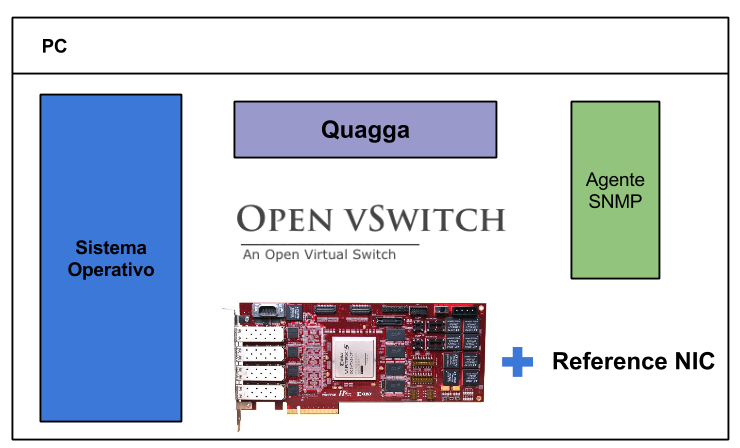
\includegraphics[width=0.7\textwidth]{Arch_Figure1}
\caption[OpenSourceRArch]{Diagrama de componentes del router open source}
\label{fig:OpenSourceRArch}
\end{figure}

Luego como puede verse en la imagen ~\ref{fig:OpenSourceRArch2}, el router open source es programado por la entidad Controlador, mediante el protocolo de comunicaci\'on OpenFlow.


\begin{figure}[htbp!] 
\centering    
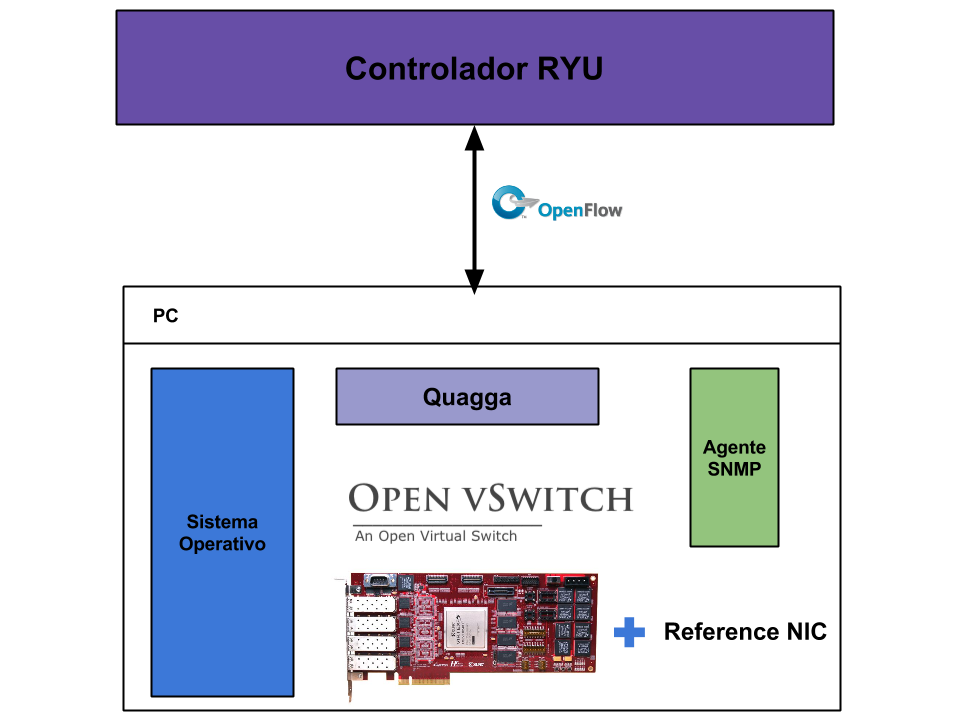
\includegraphics[width=0.7\textwidth]{Arch_Figure2}
\caption[OpenSourceRArch2]{Interacci\'on entre Router y Controlador}
\label{fig:OpenSourceRArch2}
\end{figure}

\newpage
Por otro lado enfoc\'andose en la estructura de la entidad que se dio a conocer como Controlador, vale la pena destacar solamente aquellas componentes de software; puesto que en relaci\'on al hardware, el mismo esta basado en una PC estandar. En la imagen ~\ref{fig:OpenSourceRArch3} se aprecian los componentes que constituyen al controlador.\\

Al igual que el router open source, el controlador consta de un Sistema Operativo sobre el cual posteriormente se instalan las diferentes componentes de software utilizadas. En particular el controlador se compone de un software de ruteo Quagga, un modulo encargado de sincronizar la infirmaci\'on topl\'ogica, un gerente SNMP, y finalmente el softwrare de control Ryu, sobre el cual se ejecuta el programa RauFlow encargado de implementar el plano de control de la red.

\begin{figure}[htbp!] 
\centering    
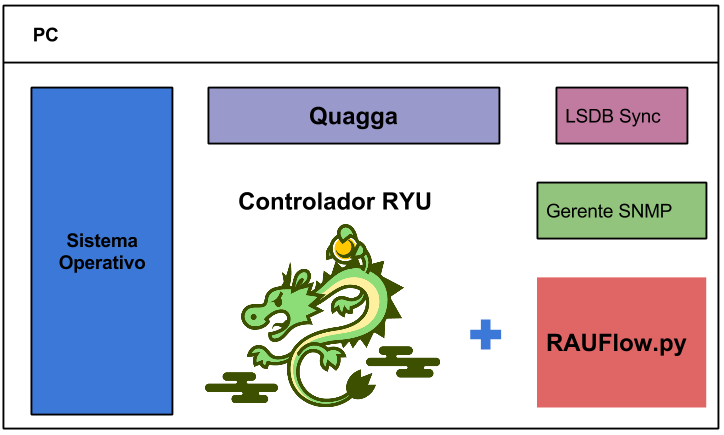
\includegraphics[width=0.6\textwidth]{Arch_Figure3}
\caption[OpenSourceRArch3]{Diagrama de componentes del Controlador}
\label{fig:OpenSourceRArch3}
\end{figure}

De esta forma, el prototipo para la nueva versi\'on de la red acad\'emica, se compone principalmente de varios nodos construidos en base al router open source, y un controlador. Como se puede observar en la imagen \ref{fig:OpenSourceRArch4} los nodos se comunican con el controlador mediante el protocolo OpenFlow como se explico con anterioridad, habilitando de esta forma a que el plano de datos sea programado por el plano de control. Por otro lado las diferentes instancias de Quagga distribu\'idas en cada nodo de la red y en el controlador, se comunican mediante el canal IP pcon el objetivo de aprender la topolog\'ia y diseminar informaci\'on de ruteo. Finalmente el gerente SNMP interactua con los diferentes agentes SNMP localizados en cada nodo mediante un canal IP, para obtener infirmaci\'on adicional acerca de cada nodo. 

\begin{figure}[htbp!] 
\centering    
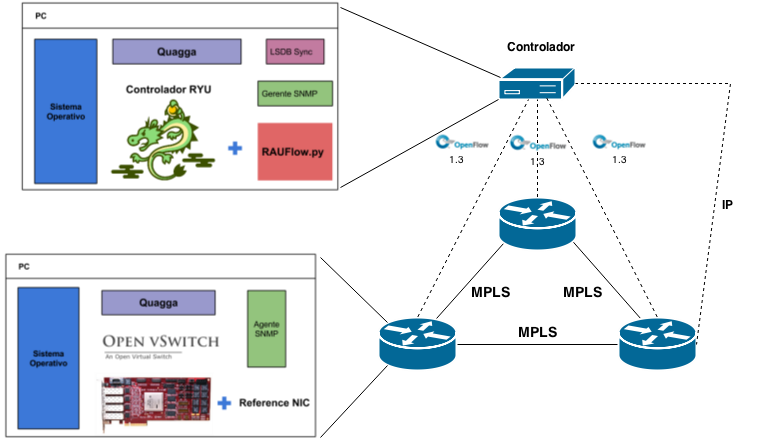
\includegraphics[width=0.9\textwidth]{Arch_Figure4}
\caption[OpenSourceRArch4]{Vista l\'ogica del prototipo}
\label{fig:OpenSourceRArch4}
\end{figure}

\section[RAUFlow]{RAUFlow}

En las secciones anteriores se ha explicado en detalle las caracter\'isticas m\'as importantes del prototipo para la nueva red acad\'emica, as\'i como las principales componentes del router open source y del controlador. No obstante, esta pendiente explicar en detalle el dise\~no de la aplicaci\'on que se di\'o a llamar RauFlow. Por ello en la siguiente secci\'on se propone un an\'alisis de dicha componente, siguiendo un proceso tradicional de Ingenier\'ia de Software, para el an\'alisis y dise\~no del mismo. La presente secci\'on consta de un apartado para el an\'alisis de los requerimientos relevados, un apartado para el relevamiento de los principales casos de uso, otro apartado donde se explica el modelo de datos alcanzado, y finalmente una apartado donde se explica en detalle la arquitectura de la aplicaci\'on.  

\subsection[An\'alisi de requerimientos]{An\'alisis de requerimientos}

Anteriormente se han descrito los requerimientos relevados sobre el prototipo pretendido por este trabajo. De ellos y de un trabajo de an\'alisis sobre la realidad modelada, se desprende la siguiente tabla de requerimientos.

\clearpage
\begin{table}[Htl]\centering
\begin{tabularx}{\textwidth}{|>{\setlength\hsize{1.0\hsize}\setlength\linewidth{\hsize}}X|}
\hline
Requerimientos Funcionales\\ \hline
\hline
\begin{itemize}
\item El Sistema debe de proveer la facilidad para obtener la informaci\'on asociada a cada nodo de la red, permitiendo a su vez agregar informaci\'on que facilite la identificaci\'on del mismo para un usuario.
\item El Sistema debe proveer la facilidad para agregar, modificar y eliminar redes virtuales. En particular al trabajar con redes virtuales se debe soportar el manejo de datos como la numeraci\'on IP del tr\'afico asociado a una red virtual, informaci\'on de capa de transporte, entre otros.
\item El Sistema debe proveer la facilidad para obtener toda la informaci\'on relevante de una red virtual.
\item El Sistema debe permitir visualizar de alguna forma los caminos existentes para el tr\'afico de una red virtual en particular, a trav\'es de la red del protot\'ipo.
\item El Sistema debe proveer la facilidad para visualizar el estado de las tablas de flujos asociadas a cualquier nodo de la red del protot\'ipo.
\end{itemize}\\
\hline
\end{tabularx}
\end{table}

\begin{table}[Htl]\centering
\begin{tabularx}{\textwidth}{|>{\setlength\hsize{1.0\hsize}\setlength\linewidth{\hsize}}X|}
\hline
Requerimientos no Funcionales\\ \hline
\hline
\begin{itemize}
\item Se debe utilizar siempre que sea posible herramientas de software libre y c\'odigo abierto.
\end{itemize}\\
\hline
\end{tabularx}
\end{table}

Teniendo en cuenta la anterior tabla de requerimientos, se realiza un relevamiento de los posibles casos de uso; llegando a un conjunto de casos de uso esenciales, los cuales se presentan en el siguiente apartado.

\subsection[Modelo de datos]{Modelo de datos}

En la figura ~\ref{fig:ModeloDeDominio} se presenta el modelo de dominio realizado a partir de la realidad a modelar. En el mismo se destacan en color amarillo aquellas entidades que se entiende se corresponden al modelado de la topolog\'ia y sus diferentes elementos como lo son los Nodos y sus Interfaces. Por otro lado en rosado se destacan aquellas entidades relacionadas al concepto de MPLS, que se consideran importante; como lo son las tablas FTN, ILM y NHLFE. Finalmente vale la pena destacar el concepto de Servicio, con el cual se decidi\'o representar a las redes virtuales soportadas en el protot\'ipo. Interesa destacar adem\'as del concepto de Servicio, que es una redefinici\'on desde una visi\'on centralizada del concepto FEC en la teor\'ia de MPLS, concepto que en la literatura de MPLS tradicional se esta vinculado a un solo nodo en una red, y no a muchos como se propone en este trabajo.  

\begin{figure}[ht!] 
\centering    
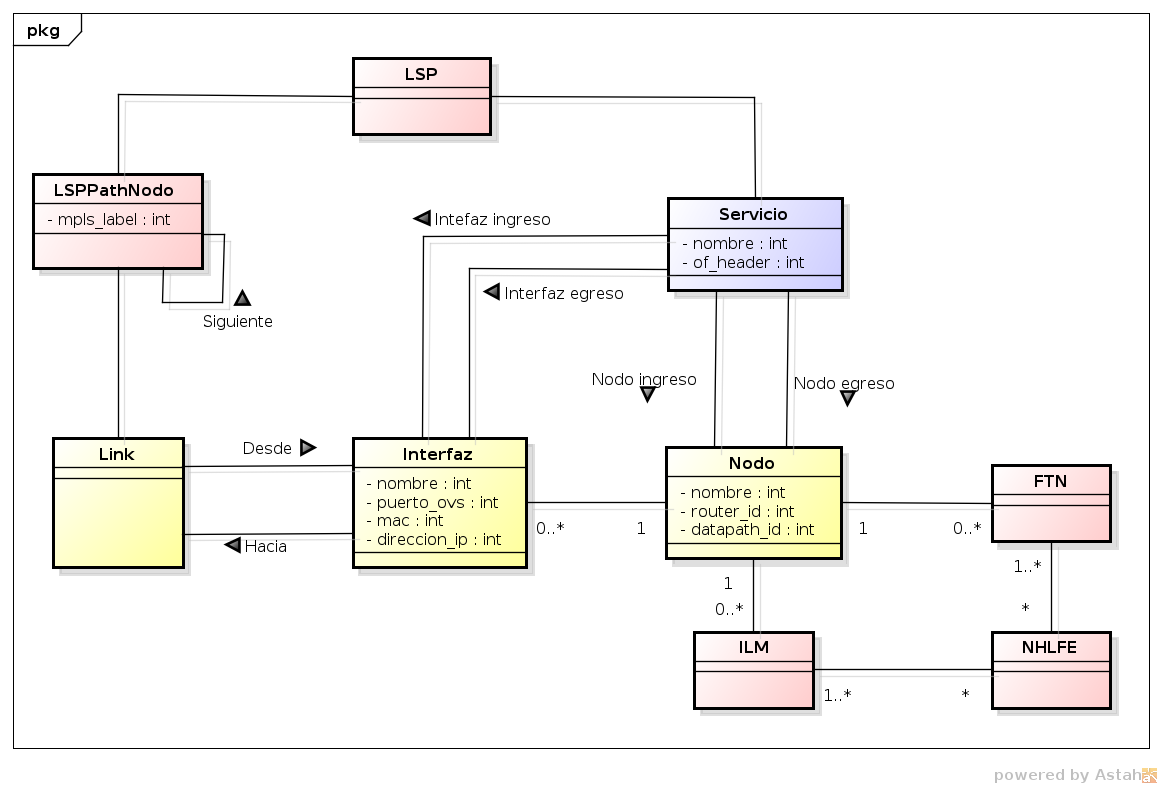
\includegraphics[width=0.7\textwidth]{Disenio_Figure1}
\caption[ModeloDeDominio]{Modelo de Dominio}
\label{fig:ModeloDeDominio}
\end{figure}

Sobre este modelo de dominio se trabaj\'o hasta llegar finalmente al diagrama de clase de dise\~no que se presenta a continuaci\'on en la figura [ref].

\newpage
\subsection[Relevamiento de casos de uso]{Relevamiento de casos de uso}

Como se menciono anteriormente se realizo un relevamiento de casos de uso inicial, del cual se desprende la lista de casos de uso que se presenta a continuaci\'on. No obstante antes de dedicarse a hablar de la misma, vale la pena resaltar que dada la complejidad de la realidad modelada, asi como la enorme existencia de una gran cantidad de funcionalidades potenciales, se debio optar por resolver en este trabajo solamente el conjunto de funcionalidades b\'asicas que permitan explorar la potencialidad de la aplicaci\'on del enfoque de SDN en la nueva versi\'on de la red acad\'emica. Sin m\'as preambulos la lista de casos de uso relevados es la siguiente:

\begin{itemize}
\item Listar Servicios
\item Agregar Servicio
\item Modificar Servicio
\item Eliminar Servicio
\item Ver Topolog\'ia
\item Ver informaci\'on b\'asica Nodo
\item Ver tabla de Flujos Nodo
\item Filtrar Lsps
\item Editar Informaci\'on extra Nodo
\item Editar Informaci\'on extra Interfaz
\end{itemize}

\newpage
\subsection[Arquitectura de RauFlow]{Arquitectura de RauFlow}

\begin{figure}[ht!] 
\centering    
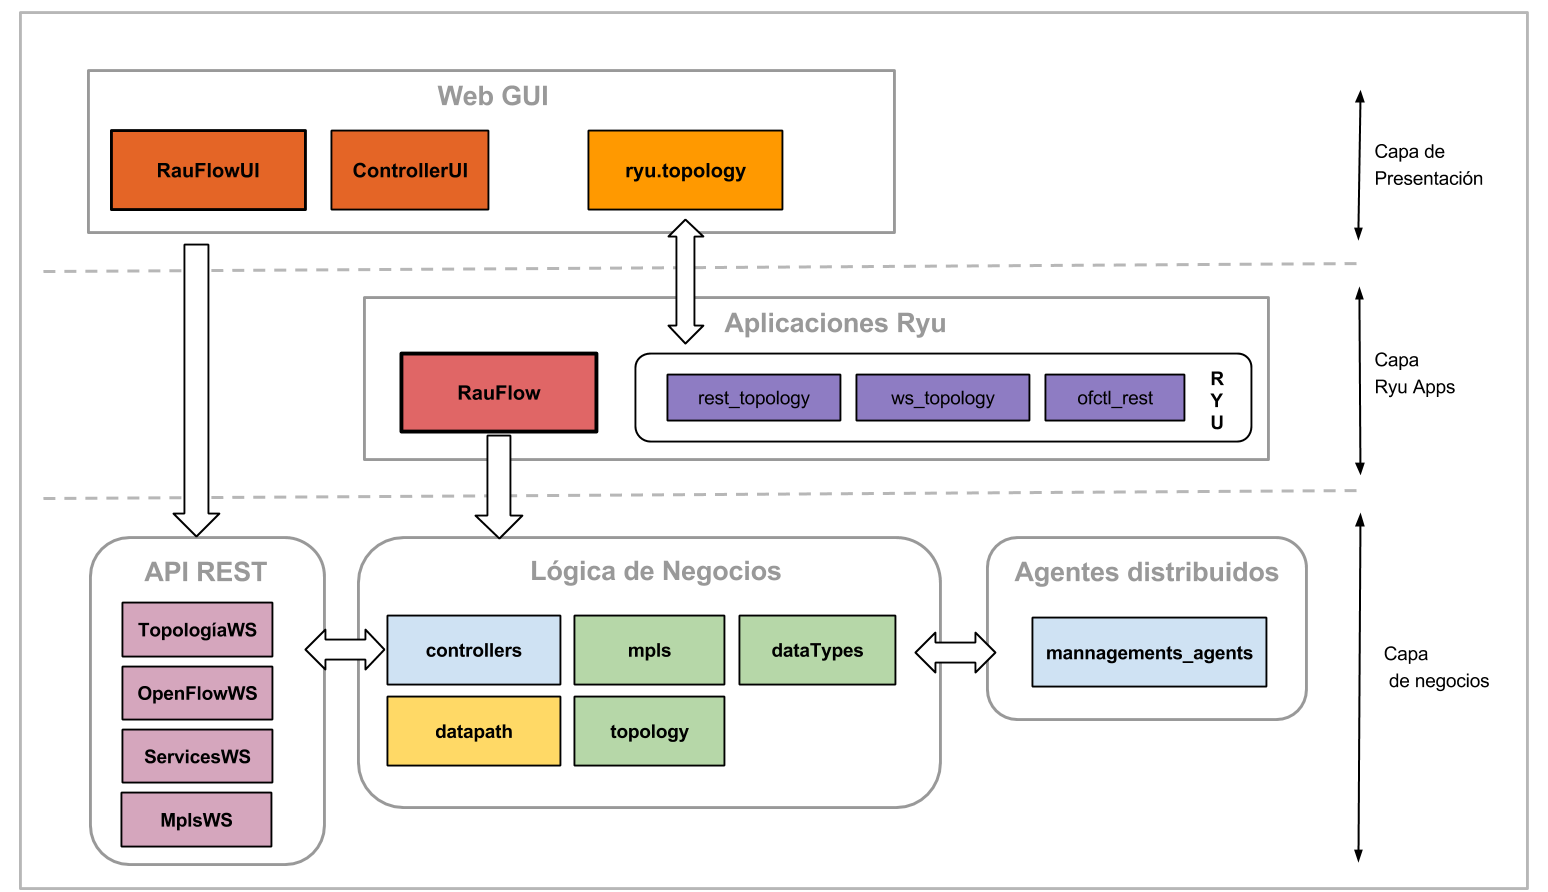
\includegraphics[width=1.0\textwidth]{Disenio_Figure2}
\caption[Diagrama de componentes]{Diagrama de componentes}
\label{fig:ModeloDeDominio}
\end{figure}

